\section{Adaptive Multimodal Diagnosis Framework}

\begin{figure*}[!t]
\centering
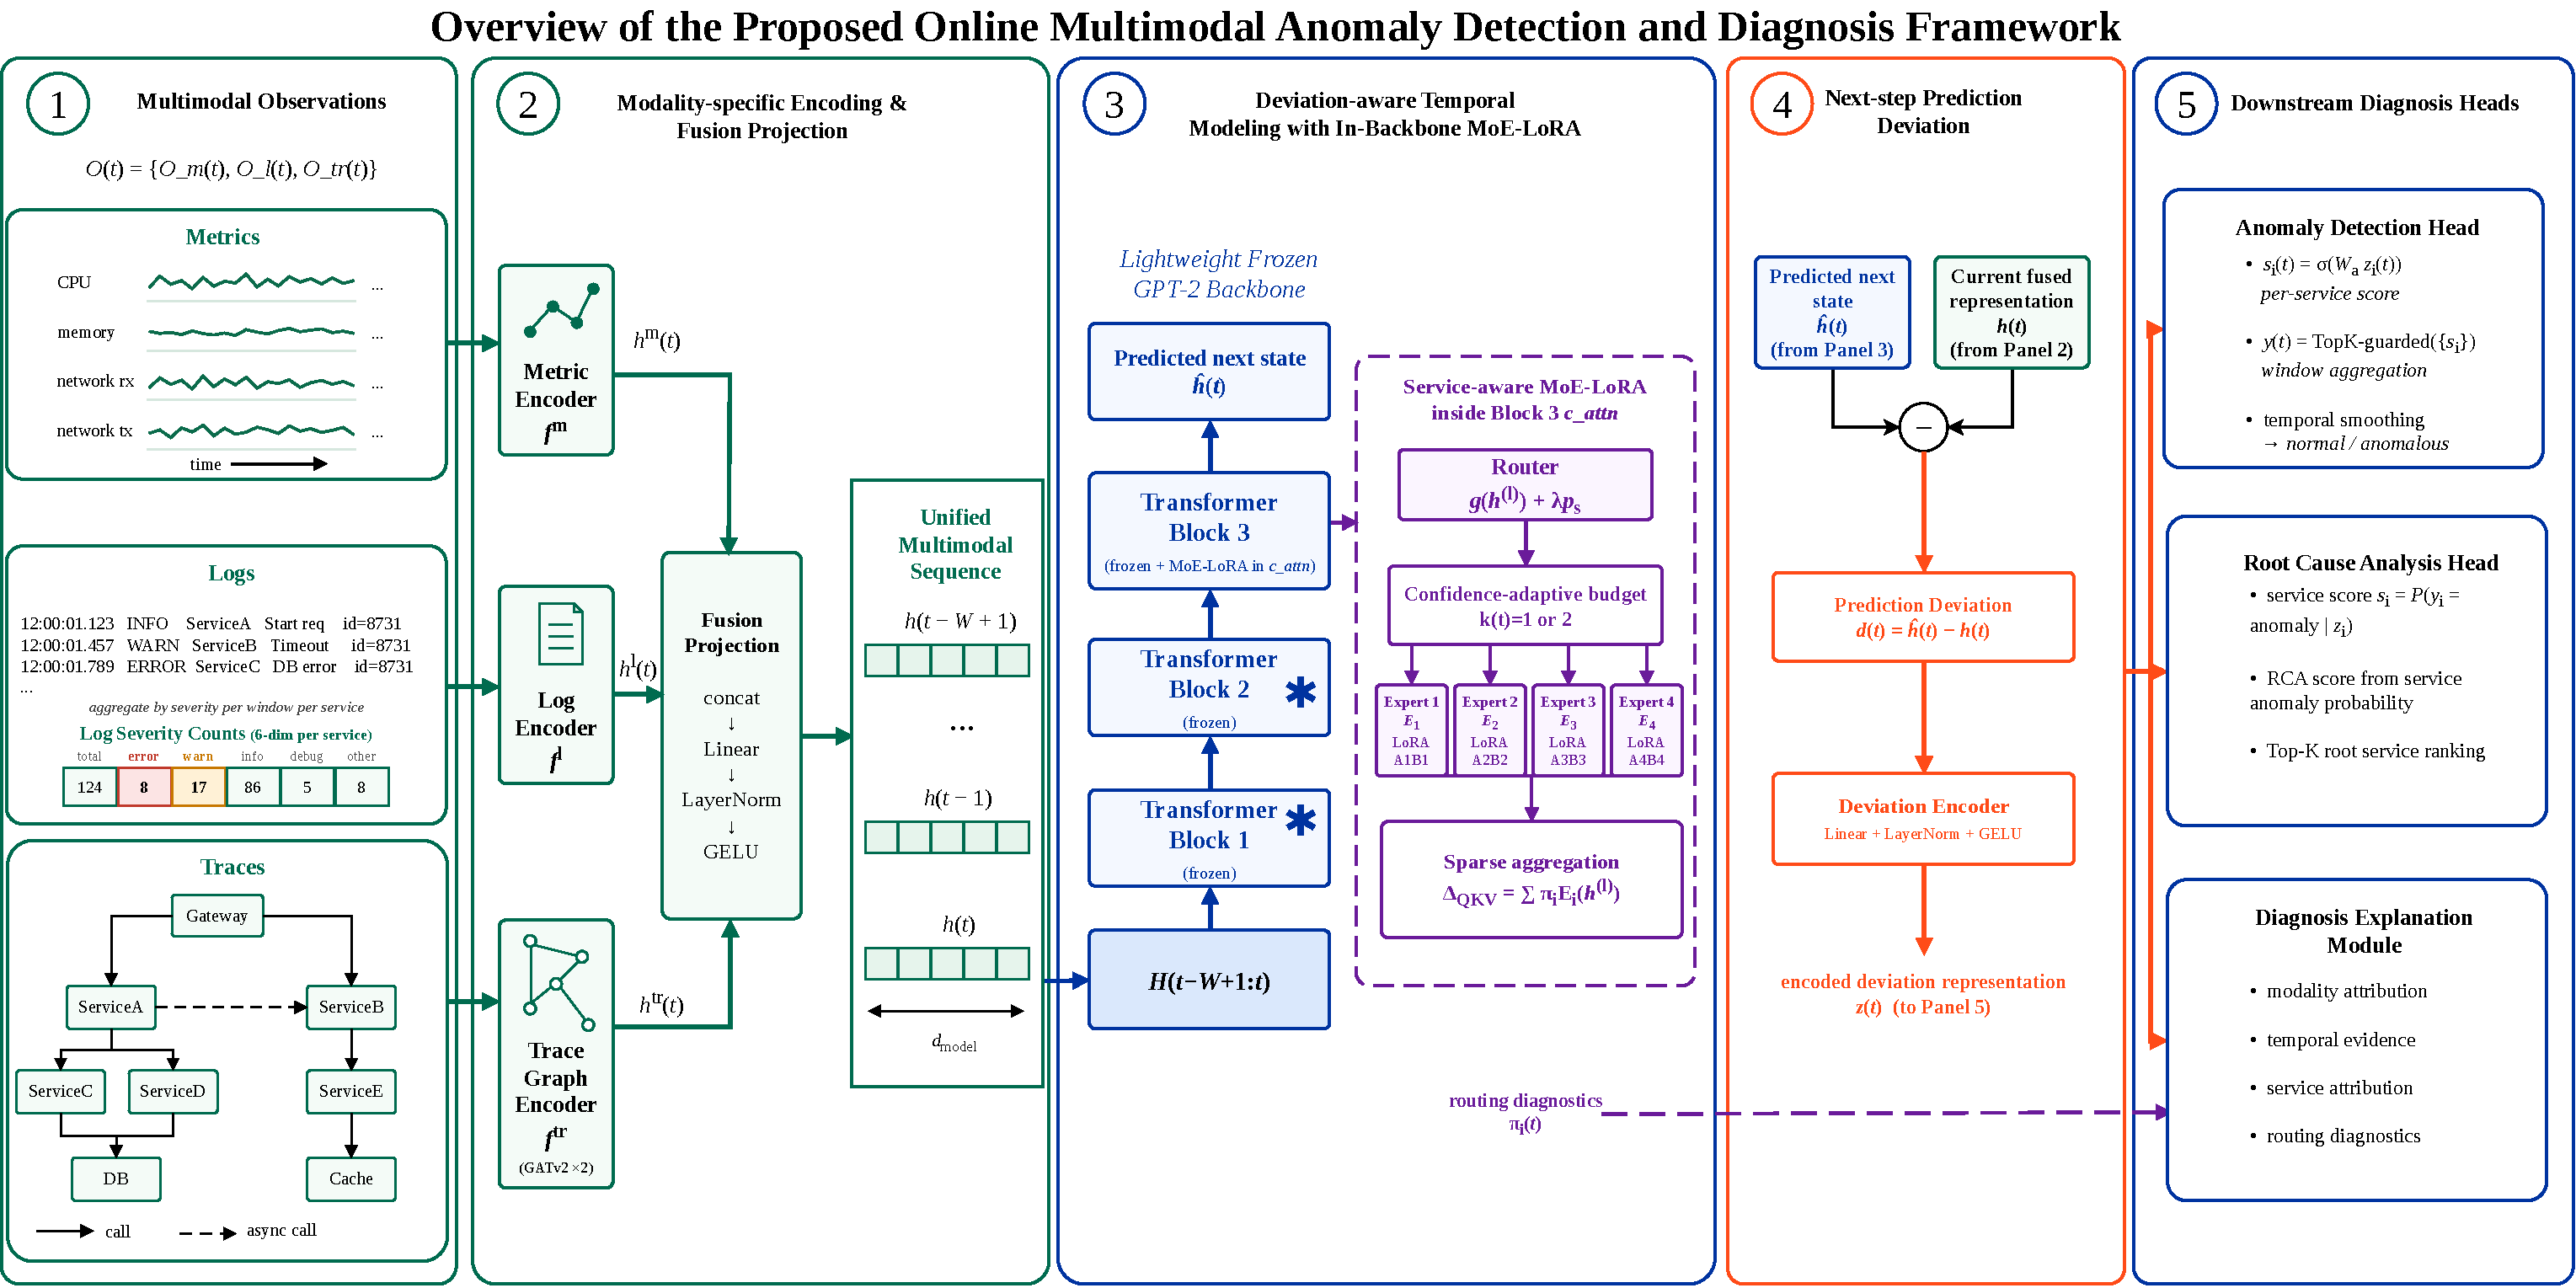
\includegraphics[width=\linewidth]{figures/asid_framework.pdf}
\caption{Overview of the proposed online multimodal anomaly detection and diagnosis framework (ASID). The framework consists of five panels: \emph{(1)} Multimodal Observations including service-level metrics, runtime logs, and inter-service traces; \emph{(2)} Modality-specific Encoding and Fusion Projection mapping each modality into a shared latent space and forming a unified multimodal sequence $\mathbf{h}_{1:W}$; \emph{(3)} Deviation-aware Temporal Modeling with a \lb{frozen truncated GPT-2 backbone} and an in-backbone service-aware MoE-LoRA adapter \lb{using a confidence-adaptive budget with at most two of four experts}; \emph{(4)} Next-step Prediction Deviation $\mathbf{d}(t)=\hat{\mathbf{h}}(t)-\mathbf{h}(t)$ encoded into a compact diagnosis representation; and \emph{(5)} Downstream Diagnosis Heads producing per-service anomaly scores, top-$K$ service ranking, and multi-dimensional diagnostic signals.}
\label{fig:framework}
\end{figure*}

To solve the above optimization problem, we design a deviation-aware multimodal diagnosis framework with adaptive sparse inference, where the sparse budget is realized through service-aware expert routing.
\subsection{Overview}

We propose an online multimodal anomaly detection and diagnosis framework, as illustrated in Fig.~\ref{fig:framework}. The framework consists of four main components:

\begin{itemize}
    \item multimodal encoding and fusion,
    \item deviation-aware temporal modeling,
    \item in-backbone adaptive sparse inference,
    \item downstream diagnosis heads.
\end{itemize}

The key idea is to construct a shared deviation representation that captures abnormal system dynamics and supports multiple diagnosis tasks.

\subsection{Multimodal Encoding and Fusion}

At each inference step, ASID receives a sliding-window tensor for each modality: service-level metrics, log-derived statistical features, and trace edge features. Each modality is encoded separately:

\begin{equation}
\mathbf{h}^{m}_{1:W} = f^{m}(\mathbf{X}^{m}_{1:W}), \quad
\mathbf{h}^{l}_{1:W} = f^{l}(\mathbf{X}^{l}_{1:W}), \quad
\mathbf{h}^{tr}_{1:W} = f^{tr}(\mathbf{X}^{tr}_{1:W}).
\end{equation}

The encoded features are fused into a unified sequence:

\begin{equation}
\mathbf{h}_{1:W} = \text{Fusion}(\mathbf{h}^{m}_{1:W}, \mathbf{h}^{l}_{1:W}, \mathbf{h}^{tr}_{1:W}).
\end{equation}
In our implementation, fusion is performed by concatenating the modality-specific embeddings at each service and time step, followed by a linear projection, layer normalization, and a GELU nonlinearity. This design keeps the fusion path lightweight while preserving modality-specific information before temporal modeling.

\subsection{Deviation-Aware Temporal Modeling}

We adopt a \lb{frozen truncated GPT-2 backbone} to model temporal dependencies and predict future system states. \lb{The efficiency goal is not that the frozen backbone has few total parameters, but that ASID concentrates adaptation into a small trainable subset while keeping the temporal representation fixed during task-specific training.}

Given the fused multimodal sequence $\mathbf{h}_{1:W-1}$ up to time $t-1$, the GPT-2 backbone autoregressively predicts the next state:

\begin{equation}
\hat{\mathbf{h}}(t) = \text{Backbone}(\mathbf{h}_{1:W-1}).
\end{equation}

We define the deviation representation as:

\begin{equation}
\mathbf{d}(t) = \hat{\mathbf{h}}(t) - \mathbf{h}(t).
\end{equation}

This deviation captures abnormal behavior and serves as a shared representation for downstream diagnosis tasks.
\subsection{Adaptive Sparse Inference}

To improve efficiency, we introduce a service-aware sparse adapter based on a mixture-of-experts (MoE) LoRA architecture. The adapter is inserted inside selected top layers of the frozen GPT-2 backbone. In our final Eadro-SN configuration, only the last GPT-2 block is adapted, and the adapter wraps the attention fused QKV projection \(c_{\mathrm{attn}}\) with lightweight LoRA experts. Thus, sparse expert routing operates inside the temporal backbone before the deviation representation is formed.

At an adapted transformer layer \(l\), the adapter routes the hidden representation \(\mathbf{h}^{(l)}(t)\) through a learned gating function augmented with a service-conditioned prior. \lb{Instead of using a fixed sparse budget at every inference step, ASID uses a confidence-adaptive budget with maximum top-\(k{=}2\). Let}

\begin{equation}
\lb{\mathbf{u}^{(l)}(t)=g(\mathbf{h}^{(l)}(t))+\lambda \mathbf{p}_{s(t)},}
\end{equation}
\begin{equation}
\lb{c^{(l)}(t)=\max_j \mathrm{softmax}(\mathbf{u}^{(l)}(t))_j ,}
\end{equation}
\begin{equation}
\lb{k^{(l)}(t)=}
\begin{cases}
\lb{1,} & \lb{c^{(l)}(t)\ge \tau_k,}\\
\lb{2,} & \lb{c^{(l)}(t)< \tau_k,}
\end{cases}
\end{equation}
\begin{equation}
\lb{\mathcal{E}^{(l)}(t)=\mathrm{Top}\text{-}k^{(l)}(t)\bigl(\mathbf{u}^{(l)}(t)\bigr).}
\end{equation}

\lb{Here \(g(\cdot)\) is a learned router, \(\mathbf{p}_{s(t)}\) is a service-specific prior vector indexed by the current service identity \(s(t)\), \(\lambda\) controls the prior strength, \(c^{(l)}(t)\) is the router top-1 confidence, and \(\tau_k\) is selected on the validation split.}

The sparse LoRA update is a weighted combination of the selected expert outputs:

\begin{equation}
\Delta^{(l)}_{QKV}(t) = \sum_{i \in \mathcal{E}^{(l)}(t)} \pi_i^{(l)}(t) \, E_i^{(l)}(\mathbf{h}^{(l)}(t)).
\end{equation}

\textbf{Latency-aware control.}
\lb{The adaptive budget \(k^{(l)}(t)\) bounds the number of LoRA experts evaluated by the adapted backbone at runtime. High-confidence router states use one expert, while uncertain states use up to two experts. Thus, ASID adapts both the active budget and the selected experts for each runtime context, while the maximum budget of two experts keeps the online execution path predictable. In the current compact deployment, this mechanism is used primarily to preserve accuracy while reducing average expert evaluations, rather than as the sole source of latency reduction.}
\subsection{Diagnosis Heads}

The deviation representation is computed per service. For each service $i$, we obtain $\mathbf{d}_i(t)$ and pass it through a shared deviation encoder to produce a compact diagnosis representation:
\begin{equation}
\mathbf{z}_i(t) = \text{Enc}(\mathbf{d}_i(t)).
\end{equation}

\textbf{Anomaly detection.}
A binary classifier converts $\mathbf{z}_i(t)$ into a per-service anomaly probability:
\begin{equation}
s_i(t) = P(\text{anomalous} \mid \mathbf{z}_i(t)) = \sigma\bigl(W_a \, \mathbf{z}_i(t)\bigr).
\end{equation}
The window-level anomaly indicator $y(t)$ is obtained by aggregating $\{s_i(t)\}$ across services through a top-$K$ guarded temporal decision module that confirms an alert only when persistently elevated scores are observed.

\textbf{Service ranking.}
For latency-critical online replay, the same per-service anomaly scores are reused for diagnostic service ranking. Services are ranked by $s_i(t)$ in descending order, and the top-$K$ ranked services are returned as the most suspicious candidates:
\begin{equation}
\text{Rank}(t) = \text{Top-}K\bigl(\{s_i(t)\}_{i=1}^{N}\bigr).
\end{equation}
This ranking-based formulation reuses the anomaly probabilities without introducing additional heads, keeping the primary inference path lightweight.

When service-level root-cause annotations are available, ASID can instantiate an auxiliary root-cause ranking branch on top of the same deviation representation. This branch estimates a rootness score \(r_i(t)\) and a victimness score \(v_i(t)\) for each service:
\begin{equation}
r_i(t)=\sigma(W_r\mathbf{z}_i(t)), \qquad
v_i(t)=\sigma(W_v\mathbf{z}_i(t)).
\end{equation}
The final root-cause ranking score is then computed as:
\begin{equation}
q_i(t)=r_i(t)-\eta v_i(t),
\end{equation}
where \(\eta\) controls how strongly likely downstream victims are suppressed. This optional root-victim disentanglement branch separates ``being anomalous'' from ``being the source of the anomaly'' and is used only in the RCA evaluation where service-level root labels are provided.

\textbf{Diagnostic signals.}
\lb{ASID reports diagnostic evidence along four dimensions computed from the same online inference pass. Modality attribution is estimated by occluding one modality at a time and measuring the positive drop in the window anomaly score. Temporal evidence is represented by the recent window-score trace and the bounded alert state used by the guarded temporal decision rule. Service-level attribution is obtained from the ranked per-service anomaly scores \(\{s_i(t)\}\). Routing diagnostics summarize the selected top-\(k\) experts, expert weights, normalized router entropy, and expert-share distribution for the suspicious services.}

\textbf{Training objective.}
ASID is trained with a supervised window-level anomaly objective on the training split, together with auxiliary terms that regularize deviation prediction and sparse routing:
\begin{equation}
\mathcal{L}
= \mathcal{L}_{\mathrm{det}}
+ \alpha \mathcal{L}_{\mathrm{pred}}
+ \gamma \mathcal{L}_{\mathrm{bal}}
+ \delta \mathcal{L}_{\mathrm{rca}}.
\end{equation}
Here \(\mathcal{L}_{\mathrm{det}}\) is binary cross-entropy for anomaly detection, \(\mathcal{L}_{\mathrm{pred}}\) penalizes next-state prediction error in the fused latent space, and \(\mathcal{L}_{\mathrm{bal}}\) discourages degenerate expert utilization. The RCA term \(\mathcal{L}_{\mathrm{rca}}\) is enabled only for the service-level root-cause ranking benchmark and combines rootness supervision with victimness regularization; for the Eadro-SN online replay experiments, \(\delta=0\). The auxiliary losses do not add computation to the online inference path.

\subsection{Limitations and Threats to Validity}

\lb{The current evaluation has several scope boundaries. The service-conditioned prior assumes that the service identity set is aligned with the training split; newly introduced or renamed services would require recalibration or incremental retraining. The overload experiment is a trace-driven single-server queue analysis rather than a full concurrent deployment benchmark.}
